%!TEX root = main.tex
%\section{Assemblage d'objets 3D sur le web avec architecture 
%événementielle}
%\label{sec:us}


\subsection{Présentation de l'expérimentation 2}
 Cette expérimentation a été réalisée sur la base du prototype 3DEvent issu des 
 travaux de Desprat et al.  
\cite{Desprat2016,Desprat2017}. Dans ces contributions, la fiabilité 
du modèle et de son implantation est soulignée de deux manières: 
\begin{itemize}
	\item fonctionnelle : manipulation et visualisation 
	3D, historique ;
	\item et technique : récupération de l'information, cohérence des 
	données, disponibilité du réseau.
\end{itemize}

L'observation du comportement des participants est 
effectuée de manière quantitative (outils de surveillance) et de manière qualitative 
(questionnaire en Annexe \ref{q:xp2}) lors de l'exécution d'une tâche 
coopérative au sein de l'application.

%The 3D data issued from X (cite) represent the different parts of a 3D printed 
%case for a camera based on RaspberryPi and a Thermal Printer. Data used in 
%the 
%experiment are triangulated surfaces converted from the STL files given. The 
%case 
%is composed of N connected components. (see figure F).

\paragraph{Tâche à effectuer}
Les participants devaient assembler les différentes parties d'un modèle \gls{3D} en 
utilisant le prototype 3DEvent (Section \ref{sec:3DEvent}) pour que le résultat 
corresponde à l'assemblage donné en exemple (images). 
La complexité de la tâche est modulée selon deux facteurs : le nombre de parties 
composant le modèle et le nombre de collaborateurs. 
Afin de permettre un apprentissage et une utilisation faciles de l'application, il a 
été choisi de conserver des manipulations 3D courantes de haut niveau pour que 
les utilisateurs les prennent en main rapidement.
%Participants had to assemble in a web-browser the different parts of a model 
%using 3DEvent application and features described in Section \ref{sec:ui} to 
%match 
%a final given assembly. The complexity of the task was modulated by the 
%number 
%of parts composing the assembly and the number of collaborators. We wanted to 
%keep the 3D manipulation tasks at high level to be easy to learn/use.
\paragraph{Population}
L'expérience a été conduite sur six groupes de deux ou trois participants chacun 
(trois groupes de deux et trois groupes de trois). 
Chaque participant était localisé en France dans une zone urbaine disposant de 
bonnes infrastructures avec une bonne connexion 
internet (au moins 20Mb/s). L'utilisation d'un réseau \gls{WAN} de bonne qualité 
permet d'éviter d'avoir des latences extrêmes (>10 secondes) au cours 
des expérimentations tout en étant dans un contexte réaliste. 
Les participants étaient des étudiants de Master ou de Doctorat en Informatique 
(pas nécessairement familiers avec les environnements 
3D). Ils étaient autorisés à communiquer entre eux.

\paragraph{Procédure}
Les modèles \gls{3D} utilisés lors de l'expérience sont décrits dans le Tableau 
\ref{table:models_xp2}. L'expérimentation se déroule en trois phases : 
\begin{enumerate}
	\item Phase \textit{Essai} : Chaque participant s'entraîne pendant 5-10 minutes 
	sur un 
	modèle de test dans l'application pour se familiariser avec l'interface et les 
	fonctionnalités proposées.
	\item Phase \textit{Solo} : Le participant effectue un assemblage du modèle 
	\textit{Rotor} ou 
	\textit{Camera Box}.
	\item Phase \textit{Collaboration} : Un groupe de participants réalise deux 
	assemblages sur 
	\begin{itemize}
		\item un petit modèle (10 ou 12 parties), 
		\item puis un plus gros modèle (16 parties).
	\end{itemize}
	La phase de collaboration a été effectuée six fois : trois fois 
	avec un groupe de deux participants et trois fois avec un groupe de trois 
	participants.
\end{enumerate}

Comme les participants pouvaient participer à différentes configurations de 
groupe durant la phase de collaboration, plusieurs modèles \gls{3D} avec des 
caractéristiques similaires (nombre de parties et nombre de triangles) ont été 
présentés pour éviter les biais liés à l'apprentissage.


\paragraph{Initialisation}

Pour chaque phase, l'application a été initialisée par le chargement des parties du 
modèle dans la bibliothèque d'objets sur chaque pair (incluant chaque 
participants). Les parties des 
objets ont volontairement été positionnées (rotation et homothétie) aléatoirement 
afin que les utilisateurs aient à manipuler les différentes fonctionnalités. Cette 
configuration nous a permis d'observer l'activité à l'intérieur de chaque groupe 
durant l'expérimentation. Chaque participant a reçu une image de l'assemblage à 
réaliser (la tâche à compléter). 

\paragraph{Données collectées}
Pour chaque expérimentation et chaque participant : le temps de réalisation, le 
nombre d'événements générés et l'horodatage de chaque événement pour 
observer le complètement de la tâche en terme de vitesse et d'efficacité ainsi 
que les effets sur le temps d'implication d'un collaborateur selon le nombre de 
collaborateurs. 

L'enregistrement des données commence lorsque le premier événement sur la 
scène initialisée est généré (horodatage du premier événement); et il s'arrête 
lorsque le groupe indique que la tâche à compléter est terminée (horodatage du 
dernier événement).


\paragraph{Questionnaire}
En dehors des données collectées, les participants devaient remplir un 
questionnaire basé sur l'expérimentation pour exprimer leurs retours qualitatifs 
concernant leur expérience (Annexe \ref{q:xp2}). 

Le questionnaire est inspiré de \cite{Lewis1995}, qui permet d'évaluer la facilité 
d'utilisation du système et l'implication dans la collaboration de chacun des 
participants. Une échelle de notation sur sept points a été utilisée, 
(1~:~pas d'accord~; 7~:~d'accord) pour avoir assez de points de discrimination \cite{Lewis1993}.
Au cours des différentes sessions collaboratives, l'application a produit plusieurs 
centaines d'événements (environ 300 par session). Les expérimentations ont été 
réalisées sur plusieurs types de dispositifs dont un \textit{smartphone} avec une 
connexion 4G. 



\subsection{Résultats et discussion}
\label{sec:res}

La Figure \ref{fig:screenshots} montre quelques captures d'écran durant une 
session collaborative sur le modèle \textit{Rotor} :  la Figure \ref{fig:ui2} montre 
l'environnement de l'utilisateur alors qu'il est en train de faire une rotation sur une 
des pales et la Figure \ref{fig:ui3} montre la réalisation d'une mise à l'échelle dans 
l'environnement 3D.
\begin{figure}[ht!]
	\centering
	
	\subfloat[Rotation (environnement \gls{3D}) et outils pour la manipulation d'objet 
	\gls{3D} 
	(panneau 
	latéral)]{\includegraphics[width=0.77\textwidth]{eps/2rotatedetail.eps}\label{fig:ui2}}\hfill
	\subfloat[Mise à l'échelle (environnement \gls{3D}) et liste des collaborateurs 
	(panneau 
	latéral)]{\includegraphics[width=0.77\textwidth]{eps/3scalecollab.eps}\label{fig:ui3}}\hfill
	\caption{Interface utilisateur pendant une session collaborative (trois 
		personnes)}{Les boîtes englobantes représentent la sélection des différents 
		collaborateurs pendant la session.}
	\label{fig:screenshots}
\end{figure}

La Figure \ref{fig:ui4} est une capture d'écran de l'interface Event Store qui montre 
les premiers événements enregistrés dans la base de données. Tous les 
événement enregistré sont nommés selon la version et le mot clé de l'agrégat 
concerné (ex: 18@scene-turbine). Cela permet de catégoriser les événements et 
de faciliter leur requête.

\begin{figure}[h!]
	\centering
	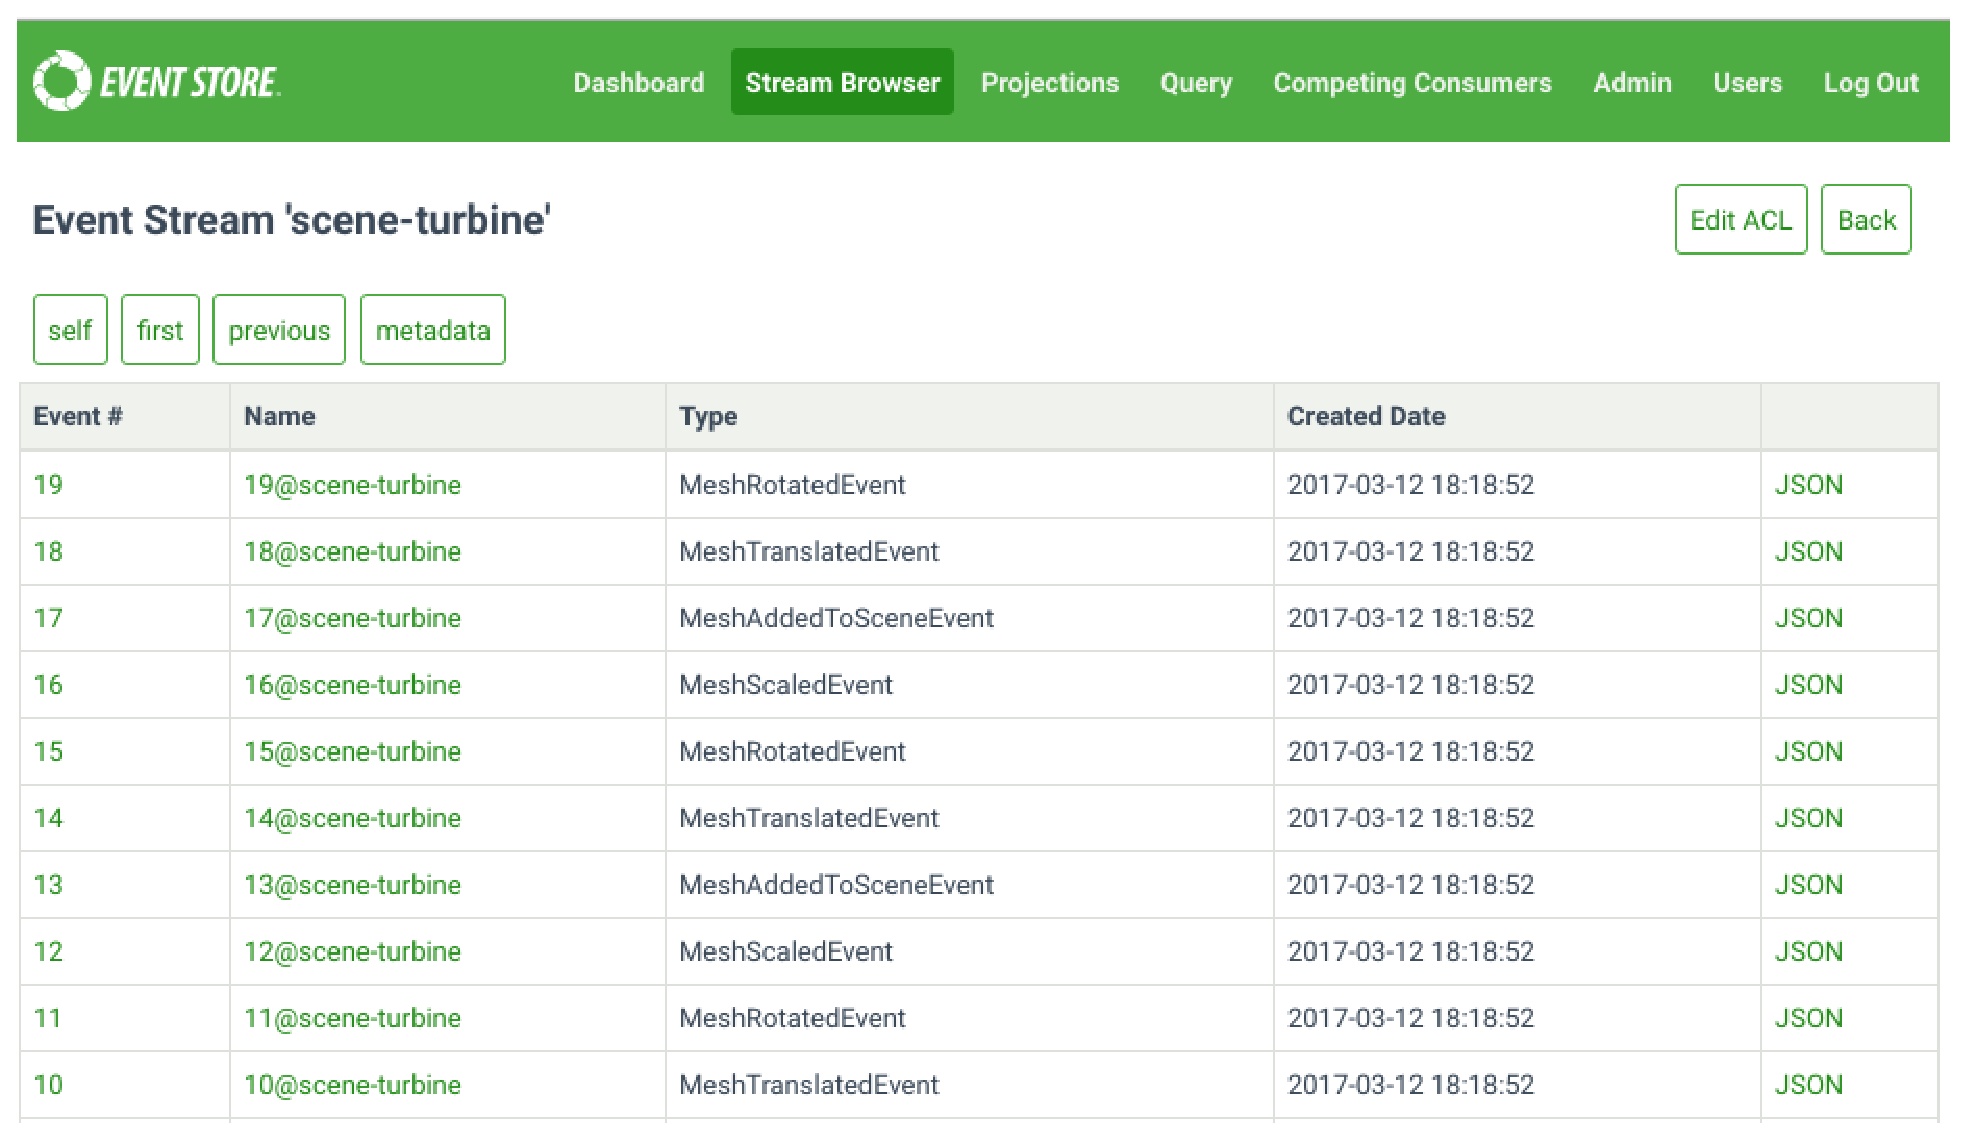
\includegraphics[width=\columnwidth]{eps/eventstore.eps}
	\caption{Persistance long-terme (Event Store\textsuperscript{\textregistered}), 
		base de données/outil de monitoring}
	\label{fig:ui4}
\end{figure}


\paragraph{Analyse des interactions}
Les traces des utilisateurs récupérées au cours des expérimentations sont la base 
du travail d'analyse présenté ci-après. Ces traces, composées d'événements 
générés par les utilisateurs, permettent de savoir qui (Figure \ref{petita}) a fait quoi 
(Figure \ref{petitb}) lors des sessions collaboratives. Généralement, le \og qui\fg{} 
est assez facile à retrouver lors de la récupération des traces. Le \og quoi\fg{} 
en revanche nécessite que les notifications aient une signification précise et proche 
du métier. Grâce au travail de découpage et de dénomination des événements 
effectué en amont, le journal d'événements (\textit{log}) indique précisément tout 
ce qui s'est passé lors de la session du point de vue du métier. Cette 
fonctionnalité est intéressante dans le contexte de la traçabilité des données et 
lors d'audits sur l'assemblage. 

\begin{figure}[]
	\centering
	
	\subfloat[Par 
	utilisateur]{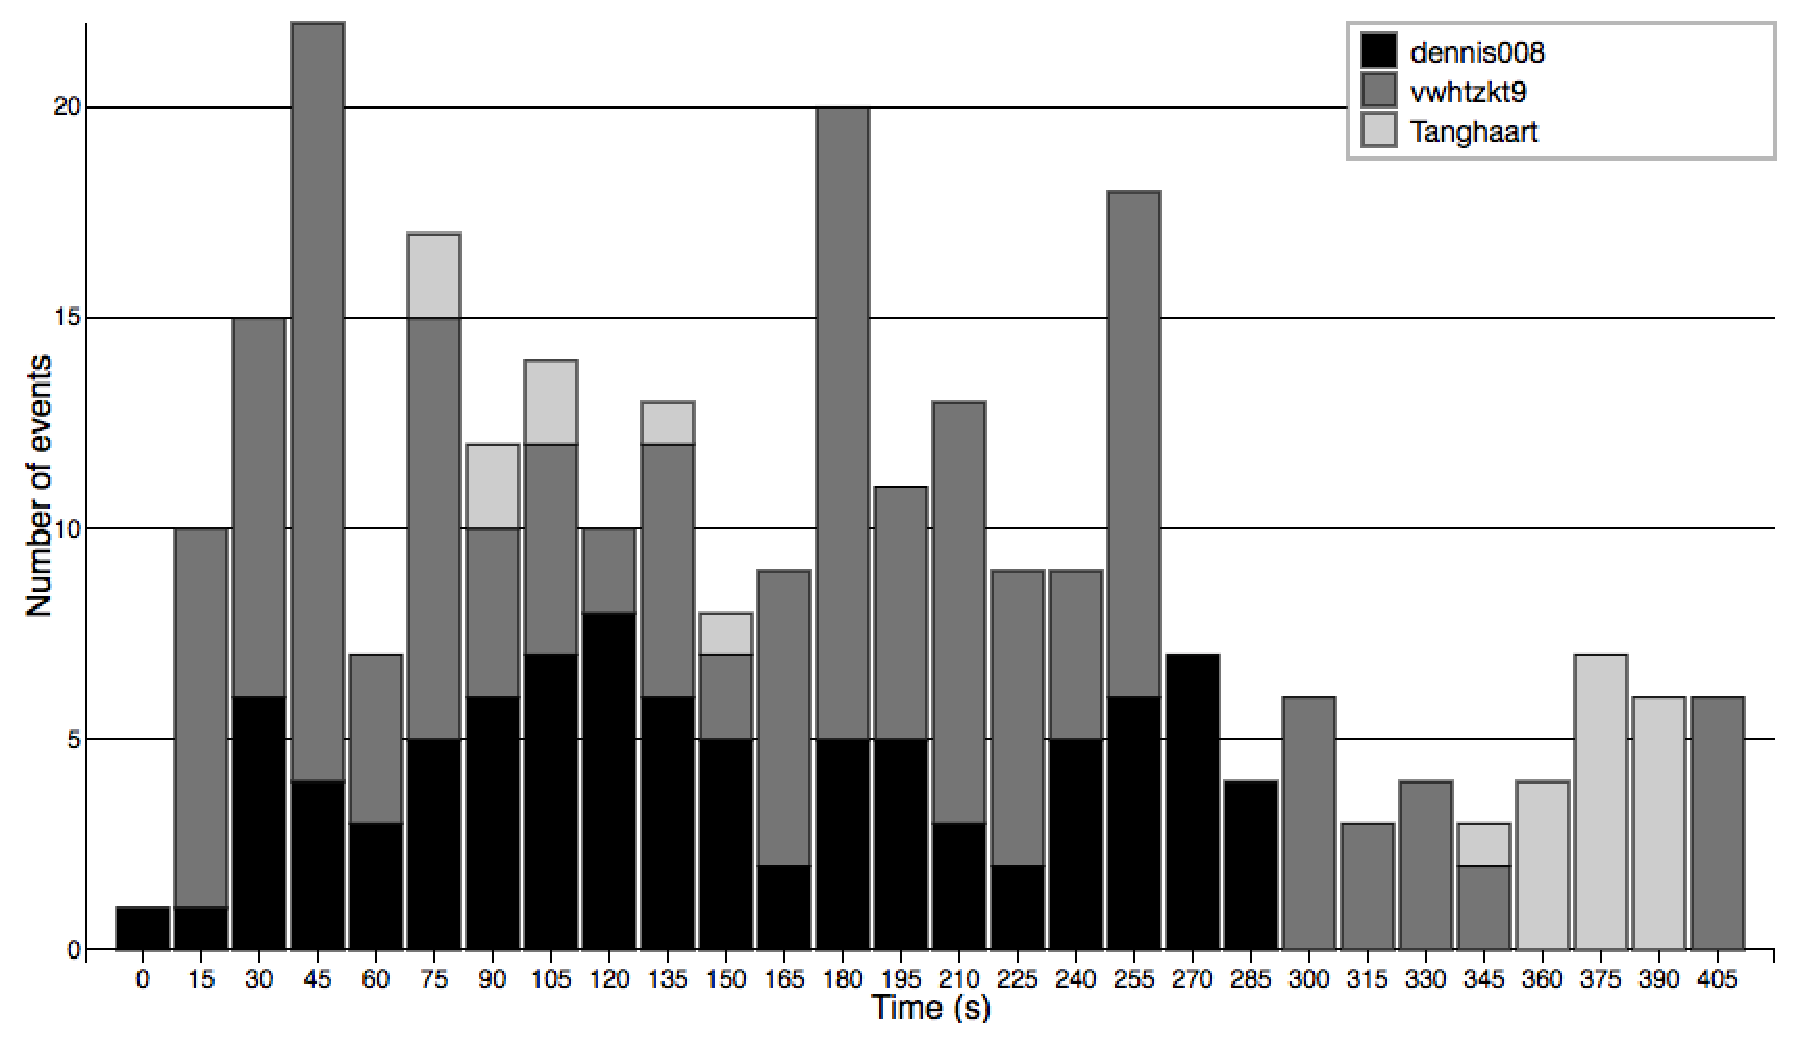
\includegraphics[width=\columnwidth]{eps/byuser.eps}\label{petita}}
	\\
	\subfloat[Par type 
	d'événement]{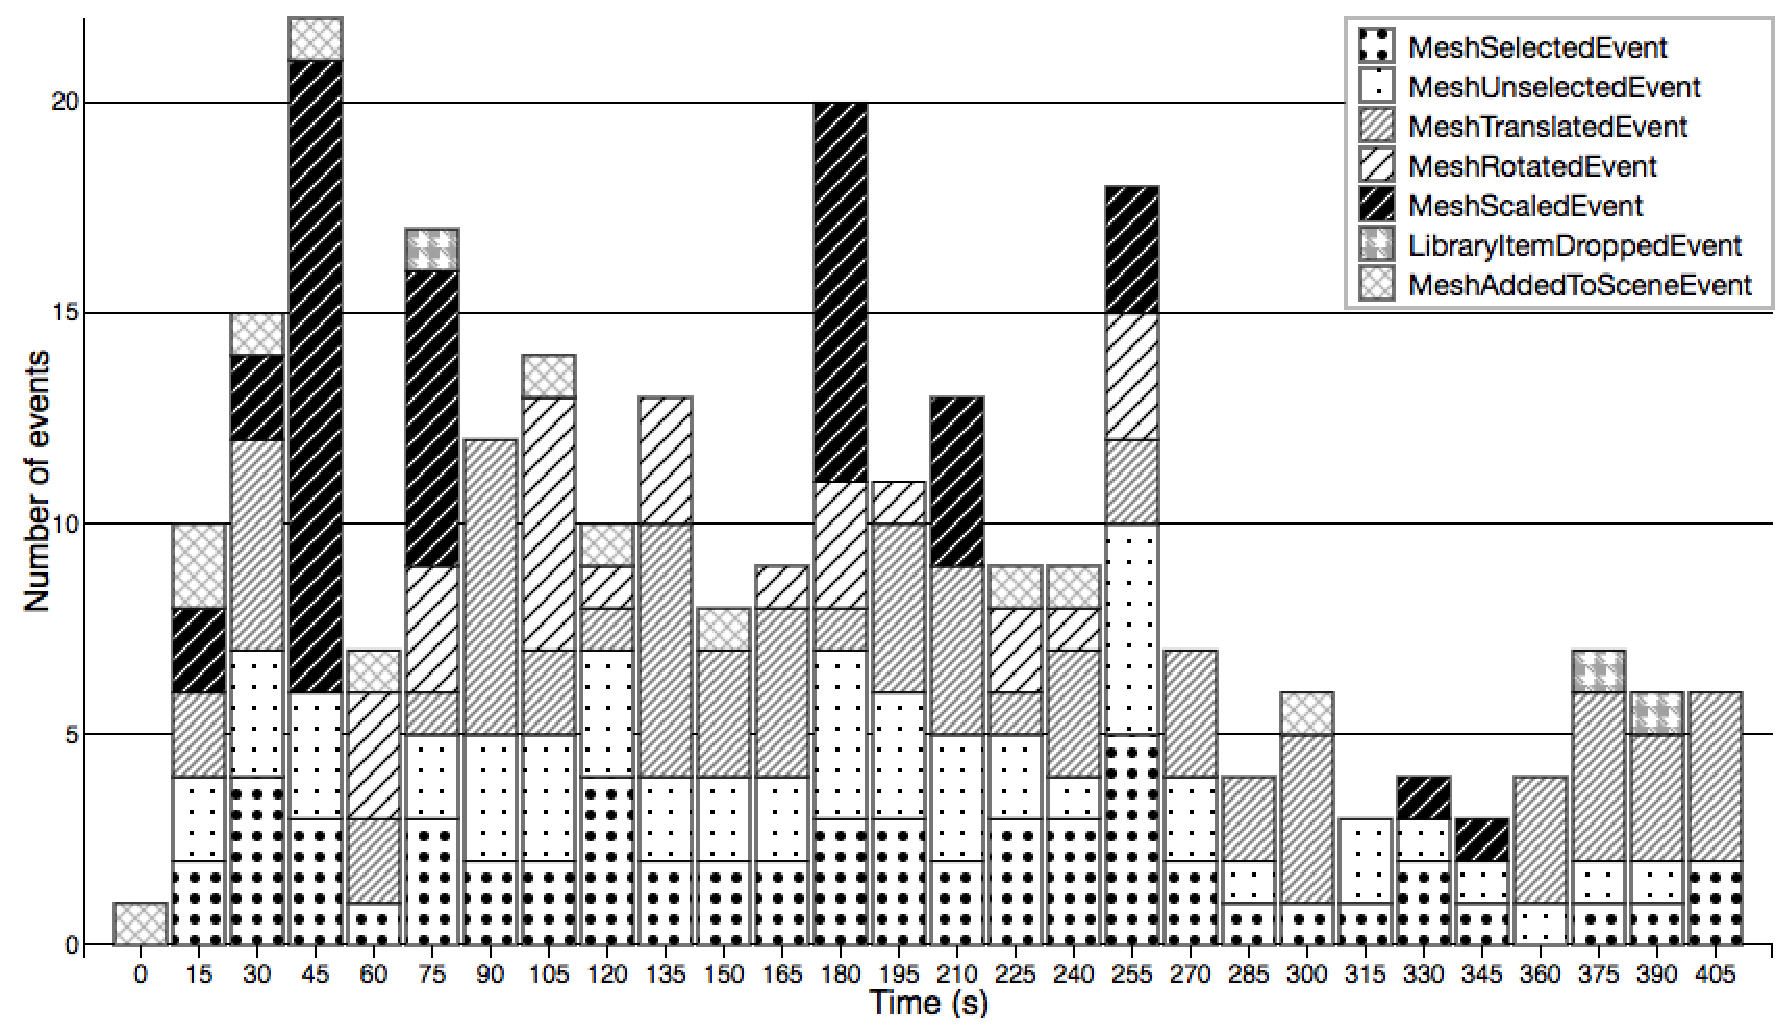
\includegraphics[width=\columnwidth]{eps/byevents.eps}\label{petitb}}
	\caption{Résumé d'une session collaborative au cours du temps}
	\label{fig:collabsession}
\end{figure}

La Figure \ref{fig:collabsession} montre deux angles d'enregistrement d'une session 
sur le modèle \textit{living room}. Au début de la session, beaucoup d'objets sont 
ajoutés (\textit{meshAddedToSceneEvent}). Seul un utilisateur a ajouté un objet 
en utilisant la fonctionnalité pour déposer un objet à un endroit spécifique de la 
scène (\textit{meshDropped}). Le nombre d'événements concernant la sélection et 
la désélection est à peu près similaire. La différence s'explique par 
le fait que l'événement de désélection n'est pas déclenché lorsque l'utilisateur 
change d'objet sélectionné. En effet, la désélection n'est pas effectuée 
explicitement par l'utilisateur. 
Dans les premiers moments, les participants ont fortement interagi 
(jusqu'à 20 événements en 15 secondes). Cela s'explique par le recours massif à 
l'ajout d'objets dans la scène pour composer le modèle et la mise à l'échelle de 
ceux-ci (causé par le positionnement arbitraire des objets de la bibliothèque). 
Ensuite, les trois utilisateurs interagissent ensemble durant quelques
minutes avant que l'un d'entre 
eux ne quitte et ne revienne quelques secondes plus tard (informations 
récupérées à partir du journal d'événements lié aux agrégats utilisateurs). Enfin, la diminution du nombre d'événements montre la fin de l'activité, les utilisateurs achevant 
la tâche et ajustant les derniers objets.

L'implication d'un utilisateur peut être perçue par le prisme de la fréquence de ses 
contributions et la variété de fonctionnalités utilisées, c.à.d. les différents 
types d'événements produits. L'analyse d'une session apporte plusieurs indicateurs 
tout au long de la session. Par exemple, l'absence d'un utilisateur pendant une 
longue période peut indiquer une déconnexion. Ou encore, l'utilisation trop 
fréquente d'un type d'événements (ou d'un motif d'événements répété) peut montrer 
une faiblesse de l'ergonomie de l'interface. Ce dernier aspect est illustré par un exemple dans la Figure \ref{petitb} à 45s, où un nombre élevé de 
MeshScaledEvent est détecté. \textit{A posteriori}, il est possible de constater  
que la fonctionnalité n'était pas suffisamment calibrée pour l'échelle du modèle et 
nécessitait plusieurs manipulations pour réaliser la bonne transformation.

	\begin{figure}[]
		\centering
		\includegraphics[width=1\columnwidth]{eps/questionnaire.eps} 
		\caption{Résultats des questionnaires collectés}
		\label{fig:questionnaire}
	\end{figure}


\paragraph{Questionnaires}
Après chaque expérimentation, le participant a rempli directement un questionnaire 
à propos de la phase \textit{Solo} et des phases \textit{Collaboration} qu'il a 
effectuées via le formulaire en ligne. Les résultats obtenus sont compilés dans la 
Figure \ref{fig:questionnaire} sous la forme de boîte à moustaches. Cette 
représentation est un moyen rapide de se figurer le profil essentiel des résultats 
des mesures quantitatives effectuées.

Globalement, les tâches ont été réalisées plus rapidement et plus efficacement 
de manière collaborative (\textit{Collaboration}) que seul (\textit{Solo}). La facilité 
d'utilisation et la simplicité de l'interface sont également soulignées positivement 
par plusieurs utilisateurs. 

Parmi les retours d'expérience négatifs, l'instabilité du réseau a parfois amené un 
peu de frustration chez certains participants. 
Cependant, les participants ont trouvé que la cohérence de l'environnement lors de 
la collaboration et la récupération des données était plus qu'acceptable. Cette 
remarque s'accompagne également du fait que la distribution des données s'est 
effectuée sans effets de bord, leur permettant de coopérer efficacement, avec peu 
de conflits détectés.

Durant l'une des expérimentations en phase \textit{Collaboration}, un 
participant a affiché à certains moments une latence de plus de 10s. ; mais 
le groupe nous a notifié que cela n'avait pas affecté la collaboration. Pour 
l'ensemble des expérimentations, quelques conflits ont été levés sur différentes 
opérations et à différents niveaux. 
Sur le réseau, la détection des conflits (mauvaise version, désynchronisation), la 
politique en place consiste à reconstruire l'état de l'application avant le conflit, i.e. 
jusqu'au dernier événement qui n'est pas en conflit, pour pouvoir resynchroniser 
les utilisateurs sur une base stable. Cette mécanique qui peut sembler 
envahissante n'a pas dérangé les utilisateurs lors de la modélisation.
Pour pallier l'absence de résolution automatique de conflit, les utilisateurs ont été 
mis a contribution dans les cas de désaccords (opérations opposées sur le même 
objet) : la résolution du conflit passe par un canal externe (chat) pour que les 
utilisateurs se mettent d'accord. Cette connaissance du métier n'est donc pas 
intégrée au système.


Dans toutes les expérimentations menées, le but a été atteint dans 
un même ordre de temps (10-12 minutes). La facilité d'utilisation du système est 
bien notée, mais il reste encore quelques aspects à améliorer notamment lors des 
désynchronisation, aucun affichage ne prévient l'utilisateur ou encore la 
sensibilisation à l'historique des objets manipulés. 
Pour modérer ces résultats, il est important de rappeler que les modèles utilisés 
ne sont pas très complexes et que tous les participants étaient débutants sur le 
système et parfois néophytes en modélisation 3D.
Le fait que l'application repose sur des technologies web a également joué en 
faveur de l'appropriation de l'application, car il a semblé assez naturel aux 
participants de se rendre à l'adresse internet donnée (sans rien installer) pour 
effectuer les tâches en manipulant un média (3D) inhabituel pour ce genre de 
plateformes. 
De plus, on peut également supposer que le prototype créé pour l'expérimentation 
correspond bien à l'objectif d'assemblage coopératif d'objets \gls{3D} puisque les 
tâches ont été réalisées rapidement. Sur une échelle de \og non-interactif \fg{} à 
\og temps réel\fg{} les participants ont qualifié l'application de \og quasi temps 
réel\fg{}. 

La satisfaction générale à propos de l'expérimentation et la satisfaction concernant 
la collaboration et l'expérience utilisateur peuvent être des indicateurs sur le fait 
que les participants ont apprécié positivement les épreuves proposées durant 
l'expérimentation. 
Quant à savoir si le nombre d'utilisateurs améliore à la fois l'efficacité et la rapidité 
du complètement de la tâche, les participants ont généralement été d'accord.

\subsection{Conclusion de l'expérimentation 2}

Les différentes phases de l'expérimentation amène le participant à prendre en 
main rapidement le prototype (Section \ref{sec:task-based-ui}). 
Le protocole, qui en proposant plusieurs épreuves sur différents modèles, offre un
large panel de situations liées aux cas d'études permettant d'évaluer les capacités 
de coordination et de coopération dans la réalisation des tâches.

L'expérimentation, construite sous l'angle de l'expérience utilisateur, propose ainsi 
d'évaluer l'utilisabilité de l'interface et les effets de l'architecture réseau choisi 
lors de l'implantation du modèle événementiel. 
Les utilisateurs ont globalement exprimé leur satisfaction concernant leur 
expérience générale : objectifs atteints, interface facile à prendre en main, 
collaboration facilitant la réalisation de la tâche. 
Concernant l'architecture réseau pour la collaboration, ils ont souligné la bonne 
récupération du système dans les cas de désynchronisation. Ces derniers 
n'apparaissent que lors d'une sélection multi-utilisateur du même agrégat et sont 
donc plutôt rares. De plus, les utilisateurs étant sensibilisés (par exemple : les 
boîtes englobantes de sélection en couleur) au fait qu'un autre utilisateur a déjà 
sélectionné l'objet, ils sont ainsi prévenus de l'occurrence potentielle de conflits. 

